% See exam.cls and examdoc.tex for the license information
\documentclass[12pt, answers]{exam}

\usepackage{amssymb}
\usepackage{makeidx}
\usepackage{amsmath}
\usepackage{graphicx}
\usepackage{caption}
\usepackage{tabulary}
\usepackage{color}
\usepackage{multicol}
\usepackage{float}
%\usepackage{multirow}
%\usepackage{enumerate}

\usepackage{array}
\newcolumntype{C}[1]{>{\centering\let\newline\\\arraybackslash\hspace{0pt}}m{#1}}

\addpoints

% In case we're not using hyperref.sty:
\providecommand{\texorpdfstring}[2]{#1}
% The following can be used in \section commands
% without generating pdf warnings:
\newcommand{\bs}{\texorpdfstring{\char`\\}{}}

\makeindex

\newcommand{\indc}[1]{\index{#1@\texttt{\char`\\#1}}}
\newcommand{\indcsub}[2]{\index{#1@\texttt{\char`\\#1}!#2}}
\newcommand{\indcstart}[1]{\index{#1@\texttt{\char`\\#1}|(}}
\newcommand{\indcstop}[1]{\index{#1@\texttt{\char`\\#1}|)}}

\newcommand{\indt}[1]{\index{#1@\texttt{#1}}}
\newcommand{\indtsub}[2]{\index{#1@\texttt{#1}!#2}}
\newcommand{\indtstart}[1]{\index{#1@\texttt{#1}|(}}
\newcommand{\indtstop}[1]{\index{#1@\texttt{#1}|)}}

\extraheadheight{-.4in}

\pagestyle{headandfoot}
%\extraheadheight{.2 in}
\firstpageheader{}{}{}
\runningheader{}{}{}
\firstpagefooter{}{Database search}{Page \thepage\ of \numpages}
\firstpagefootrule
\runningfooter{}{Database search}{Page \thepage\ of \numpages}
\runningfootrule

%---------------------------------------------------------------------

\shadedsolutions
%\noprintanswers
\definecolor{SolutionColor}{rgb}{0.8,0.9,1}

\setcounter{section}{4}

\begin{document}

\section{Exercises -- Database search}

%---------------------------------------------------------------------
\begin{questions}

%%% Question 1
\question \textbf{N-grams}
  
N-grams are n-letter words that can be used for database search methods. Create a table of 2-grams for q: ATGCAT.

\vspace{0.1 in}

\begin{parts}

%% (a)
  \part List all 2-grams of q.

\begin{solution}[0.5 in]
\begin{verbatim}
  AT, TG, GC, CA, AT
\end{verbatim}
\end{solution}

%% (b)
\part Fill the table with the 2-grams and the corresponding indices of q.

\begin{figure}[H]
      \centering
      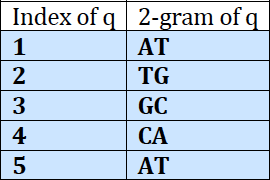
\includegraphics[width=0.25 \textwidth]{fig05/n-gram_solution.png}
\end{figure}

\end{parts}


\newpage

%%% Question 2
\question \textbf{Matching n-grams}
  
Calculate the scores of the segment pairs between q: CG and all 2-gram permutations of \{A, C, G, T\}.

\medskip 

Score matrix:
\begin{figure}[H]
      \centering
      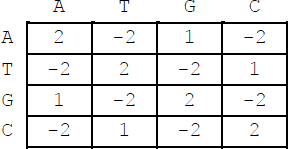
\includegraphics[width=0.25 \textwidth]{fig05/score_scheme_1.png}
\end{figure}

\vspace{0.1 in}

\begin{parts}

%% (a)
  \part Fill the scores between CG and all its matching n-grams.

\begin{figure}[H]
      \centering
      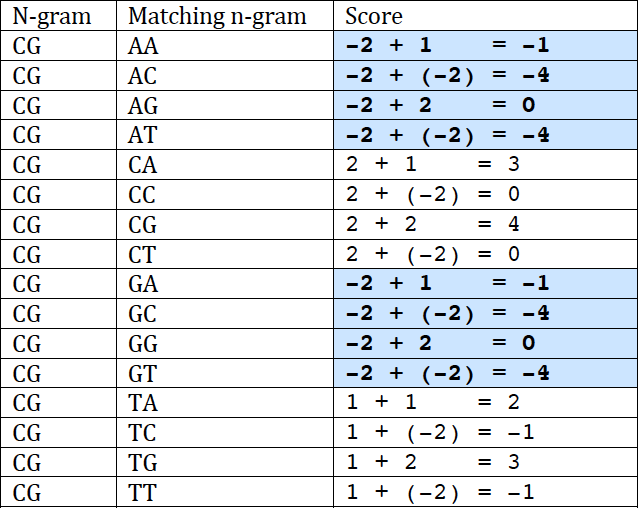
\includegraphics[width=0.6 \textwidth]{fig05/matching_n-gram_solution.png}
\end{figure}

%% (b)
\part Identify all matching n-grams when the threshold value T is 3.

\begin{solution}[0.5 in]
\begin{verbatim}
  CA, CG, TG
\end{verbatim}
\end{solution}

\end{parts}


\newpage

%%% Question 3
\question \textbf{Lookup table for n-grams}
  
Create a 2-gram lookup table with indices and scores for the sequence q: ATGCAT. 

\medskip 

Score matrix:
\begin{figure}[H]
      \centering
      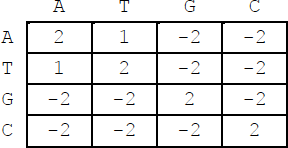
\includegraphics[width=0.25 \textwidth]{fig05/score_scheme_2.png}
\end{figure}

 T: 3 \\

Pre-calculated scores of all segment pairs:
\begin{figure}[H]
      \centering
      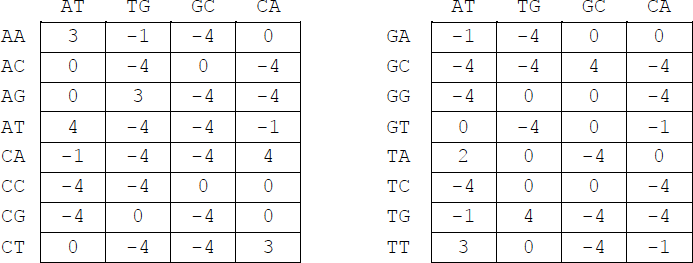
\includegraphics[width=0.65 \textwidth]{fig05/lookup_table_precalculated.png}
\end{figure}

\begin{parts}

%% (a)
  \part Fill the table.

\begin{figure}[H]
      \centering
      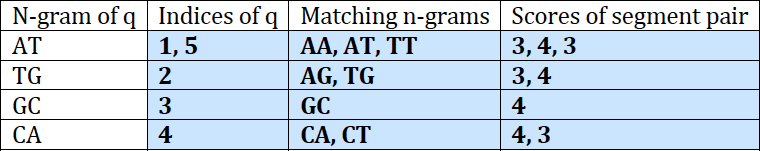
\includegraphics[width=0.65 \textwidth]{fig05/lookup_table_n-gram_solution.png}
\end{figure}

%% (b)
\part Create a lookup table for the matching n-grams with scores and indices.

\begin{figure}[H]
      \centering
      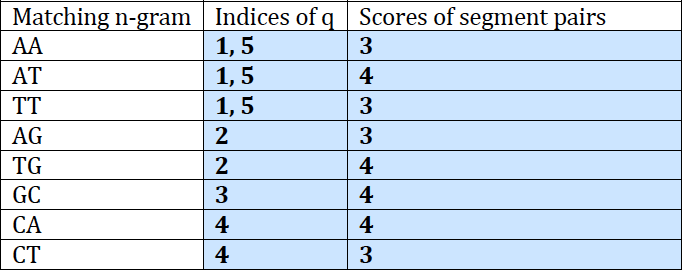
\includegraphics[width=0.6 \textwidth]{fig05/lookup_table_n-gram_final_solution.png}
\end{figure}

\end{parts}

\end{questions}
%---------------------------------------------------------------------
       
\end{document}

